%
%===============>>  ГРУППА 11-2 МОДУЛЬ 4  <<=============
%
\setmodule{4}
%
%===============>>  Занятие 1  <<===============
%
\begin{class}[number=1]
	\begin{listofex}
		\item Взято из Решу ЕГЭ
	\end{listofex}
\end{class}
%
%===============>>  Занятие 2  <<===============
%
%\begin{class}[number=2]
%	\begin{listofex}
%		\item Пусто
%	\end{listofex}
%\end{class}
%
%===============>>  Домашняя работа 1  <<===============
%
%\begin{homework}[number=1]
%	\begin{listofex}
%		\item Пусто
%	\end{listofex}
%\end{homework}
%
%===============>>  Занятие 3  <<===============
%
\begin{class}[number=3]
	\textbf{(!) Запомнить:} если нужно найти точку максимума или минимума --- ищем \( x \), а если нужно найти наибольшее или наименьшее значение --- ищем \( y \).
\begin{listofex}
	\item Найдите точку минимума функции \( y=x^3-3x^2+2 \).
	\item Найдите наименьшее значение функции \( y=x^3-3x^2+2 \) на отрезке \( [1;4] \).
	\item Найдите точку минимума функции \( y=x^3+5x^2=7x-5 \).
	\item Найдите наименьшее значение функции \( y=\dfrac{x^3}{3}-9x-7\sin30\degree \) на отрезке \( [-3;3] \).
	\item Найдите наибольшее значение функции \( y=\dfrac{x^2+25}{x} \) на отрезке \( [-10;-1] \).
	\item Найдите точку минимума функции \( y=-\dfrac{x}{x^2+1} \).
	\item Найдите точку минимума функции \( y=(x+16)e^{x-16} \).
	\item Найдите точку максимума функции \( y=(x^2-10x+10)e^{5-x} \).
	\item Найдите наименьшее значение функции \( y=(x+3)^2e^{-3-x} \) на отрезке \( [-5;-1] \).
	\item Найдите наименьшее значение функции \( y=(3x^2-36x+36)e^{x-10} \) на отрезке \( [8;11] \).
	\item Найдите наименьшее значение функции \( y=(x+3)^2(x+5)-1 \) на отрезке \( [-4;-1] \).
	\item Найдите наибольшее значение функции \( y=\ln(x+5)^5-5x \) на отрезке \( [-4,5;0] \).
	\item Найдите наибольшее значение функции \( y=\ln(11x)-11x+9 \) на отрезке \( \left[ \dfrac{1}{22};\dfrac{5}{22} \right] \).
	\item Найдите точку минимума функции \( y=3x-\ln(x+3)^3 \).
	\item Найдите наименьшее значение функции \( y=e^{2x}-6e^x+3 \) на отрезке \( [1;2] \).
	\item Найдите наименьшее значение функции \( y=3+\dfrac{5\pi}{4}-5x-5\sqrt{2} \) на отрезке \( \left[ 0;\dfrac{\pi}{2} \right] \).
	\item Найдите наименьшее значение функции \( y=5\cos x - 6x+4 \) на отрезке \( \left[ -\dfrac{3\pi}{2};0 \right] \).
	\item Найдите наименьшее значение функции \( y=4\tg x - 4x - \pi + 5 \) на отрезке \( \left[ -\dfrac{\pi}{4};\dfrac{\pi}{4}\right] \).
	\item Найдите точку максимума функции \( y=\sqrt{4-4x-x^2} \).
	\item Найдите точку максимума функции \( y=\log_2(2+2x-x^2)-2 \).
	\item Найдите точку минимума функции \( y=11^{x^2-6x} \).
	\item 
	\begin{minipage}[t]{0.67\textwidth}
		На рисунке изображены графики функций \( f(x)=k\sqrt{x} \). Найдите \( f(6,76) \).
	\end{minipage}
	\begin{minipage}[c]{0.25\textwidth}
		\includegraphics[align=t, width=\textwidth]{./pics/G102M4L3-2}
	\end{minipage}
	\item При адиабатическом процессе для идеального газа выполняется закон \( pV^k=1,25 \cdot 10^8 \) Па\( \cdot \)м\( ^4 \), где \( p \) – давление газа (в Па), \( V \) – объём газа (в м\( ^3 \)), \( k=\dfrac{4}{3}\). Найдите, какой объём \( V \) (в м\( ^3 \)) будет занимать газ при давлении \( p \), равном \( 2 \cdot 10^5 \) Па.
	\item Решите уравнение \( \sqrt{x^3-4x^2-10x+29}=3-x \).\\
	\textbf{(!)} Для решения этого уравнения воспользуйтесь равносильным переходом:
	\[ \sqrt{f}=g
	\Rightarrow
	\left\{
	\begin{array}{l}
		f=g^2,\\
		g\ge0.
	\end{array}
	\right. \]
\end{listofex}
\end{class}
%
%===============>>  Занятие 4  <<===============
% смещение на одно занятие с прошлого месяца
%\begin{class}[number=4]
%	\begin{listofex}
%		\item Пусто
%	\end{listofex}
%\end{class}
%
%===============>>  Домашняя работа 2  <<===============
%
%\begin{homework}[number=2]
%	\begin{listofex}
%
%	\end{listofex}
%\end{homework}
%
%===============>>  Занятие 5  <<===============
% смещение на одно занятие с прошлого месяца
\begin{class}[number=5]
	\begin{listofex}
		\item
		\begin{minipage}[t]{\bodywidth}
			На рисунке изображён график функции вида \[ f(x)=ax^2+bx+c, \] где числа \(a, b, c\) --- целые. Найдите значение \(f(6,5)\).
		\end{minipage}
		\hspace{0.05\linewidth}
		\begin{minipage}[t]{\picwidth}
			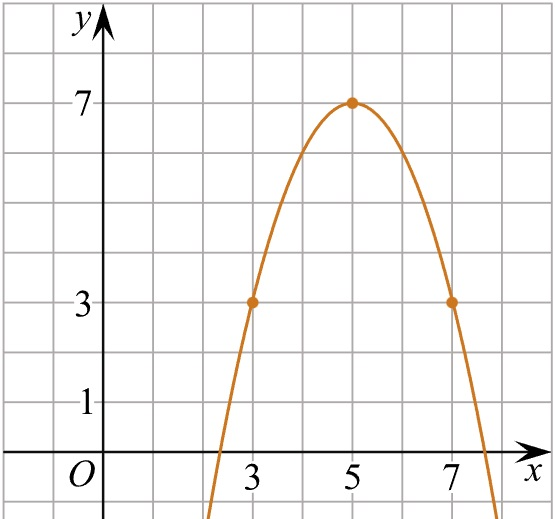
\includegraphics[align=t, width=\textwidth]{pics/G101M4H2-5.jpg}
		\end{minipage}
		\item
		\begin{minipage}[t]{\bodywidth}
			На рисунке изображён график функции вида \[ f(x)=\dfrac{k}{x+b}+a, \] где числа \(a, b, c\) --- целые. Найдите \(f(9)\).
		\end{minipage}
		\hspace{0.05\linewidth}
		\begin{minipage}[t]{\picwidth}
			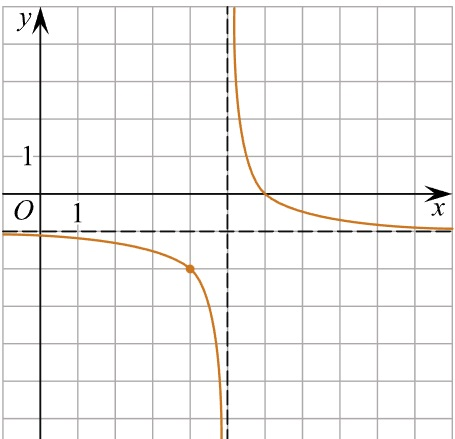
\includegraphics[align=t, width=\linewidth]{pics/G101M4C5-2.jpg}
		\end{minipage}
		\item
		\begin{minipage}[t]{\bodywidth}
			На рисунке изображён график функции вида \[ f(x)=\dfrac{k}{x+b}+a, \] где числа \(a, b, c\) --- целые. Найдите \(f(4)\).
		\end{minipage}
		\hspace{0.05\linewidth}
		\begin{minipage}[t]{\picwidth}
			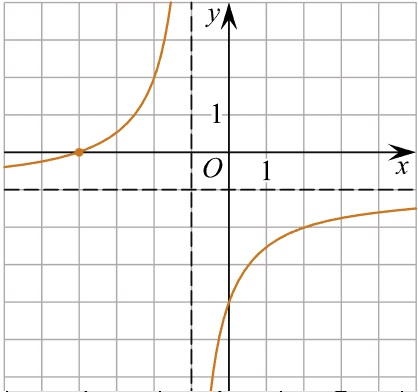
\includegraphics[align=t, width=\linewidth]{pics/G101M4C5-3.jpg}
		\end{minipage}
		\item
		\begin{minipage}[t]{\bodywidth}
			На рисунке изображён график функции вида \[ f(x)=ax+|bx+c|+d, \] где числа \(a, b, c, d\) --- целые.\\ Найдите корень уравнения \(ax+d=0\).
		\end{minipage}
		\hspace{0.05\linewidth}
		\begin{minipage}[t]{\picwidth}
			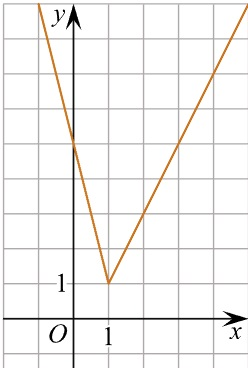
\includegraphics[align=t, width=\linewidth]{pics/G101M4C5-6.jpg}
		\end{minipage}
		\item В прямоугольном треугольнике угол между высотой и биссектрисой, проведенными из вершины прямого угла, равен \( 21\degree \). Найдите меньший угол данного треугольника. Ответ дайте в градусах.
		\item В треугольнике \( ABC \) \( AC = BC \), \( AB = 10 \), высота \( AH \) равна \( 3 \). Найдите синус угла \( BAC \).
		\item В треугольнике \( ABC \) угол \( C \) равен \( 90\degree \), \( AC=4,8 \) и \( \sin\angle A = \dfrac{7}{25} \). Найдите \( AB \).
		\item В треугольнике \( ABC \) угол \( C \) равен \( 90\degree \), \( CH \) --- высота, \( BC=3 \), а \( \sin A=\dfrac{1}{6} \). Найдите \( AH \).
		\item В треугольнике \( ABC \) угол \( C \) равен \( 90\degree \), высота \( CH=4 \), \( BC=8 \). Найдите \( \cos A \).
		\item Острый угол прямоугольного треугольника равен \( 32\degree \). Найдите острый угол, образованный биссектрисами этого и прямого углов треугольника. Ответ дайте в градусах.
		\item В прямоугольном треугольнике острые углы относятся как \( 1:2 \), а больший
		катет равен \( 4\sqrt{3} \). Найти радиус окружности, описанной около треугольника.
		\item На катете \( AC \) прямоугольного треугольника \( ABC \) как на диаметре построена окружность, пересекающая гипотенузу \( AB \) в точке \( K \). Найдите \( CK \), если \( AC = 2 \) и \( \angle A = 30\degree \).
		\item Докажите, что угол между биссектрисами двух смежных углов прямой.
		\item Окружность касается двух параллельных прямых и их секущей. Докажите, что отрезок секущей, заключенный между параллельными прямыми, виден из центра окружности под
		прямым углом.
		\item В треугольнике \( ABC \) к стороне \( AC \) проведены высота \( BK \) и медиана \( MB \), причем \( AM =BM \). Найдите косинус угла \( KBM \), если \( AB=1 \), \( BC = 2 \).
	\end{listofex}
\end{class}
%
%===============>>  Домашняя работа 3  <<===============
%
%\begin{homework}[number=2]
%	\begin{listofex}
%
%	\end{listofex}
%\end{homework}
%\newpage
%\title{Подготовка к проверочной работе}
%\begin{listofex}
%	
%\end{listofex}
%
%===============>>  Занятие 7  <<===============
%
%\begin{class}[number=7]
%	\begin{listofex}
%	
%	\end{listofex}
%\end{class}
%
%===============>>  Провечная работа  <<===============
%
%\begin{exam}
%	\begin{listofex}
%	
%	\end{listofex}
%\end{exam}